\documentclass[latex/main.tex]{subfiles}

\begin{document}
\section{Simulations}\label{sec:simulations}

\subsection{Simulation Settings}
Monte Carlo simulations with $N = 10,000$ replications were used to evaluate time- and autocorrelation-domain methods. Time series realizations $x_t = \{x_1, x_2, ..., x_T\}$ with $T=4800$ were based on three data-generating processes, each characterized by a different autocorrelation structure: AR1, AR2, and autocorrelations derived from rfMRI data. All autocorrelation structures shared the same AR1 projection ($\phi_\text{AR1}$) for comparable timescales. That is, there is always a $\phi_\text{AR1}$ value that represents the AR1 projection, even if the time series was generated by a more complex process. To define a feasible parameter range for simulation, we referred to the Human Connectome Project dataset, where $\hat\phi_\text{AR1}$ estimates ranged from +0.1 to +0.8. Accordingly, autocorrelation strength was varied using five positive $\phi_\text{AR1}$ values (0.1 to 0.8) with corresponding timescales $\tau_\text{AR1}$ from equation \eqref{eq:ar1-tau}. This design resulted in a total of 15 simulation settings (three data-generating models $\times$ five autocorrelation strengths). For each setting, estimator performance was assessed by relative root mean squared error: 

\begin{align}
    \text{rRMSE}(\hat\tau) = \frac{\sqrt{\frac{1}{N} \sum_{n=1}^N (\hat\tau_n - \tau)^2}}{\tau}, \quad \text{rRMSE}(\widehat{\text{se}}(\hat\tau)) = \frac{\sqrt{\frac{1}{N} \sum_{n=1}^N \left(\widehat{\text{se}}(\hat\tau_n) - \text{se}(\hat\tau)\right)^2}}{\text{se}(\hat\tau)}.
\end{align}

\subsubsection{Time-Domain Simulations}
In the \textit{AR1 setting}, the data-generating process matches the fitted model, with time series simulated from an AR1 model:
\begin{align}
    x_t &= \phi x_{t-1} + e_t, \quad e_t \overset{\text{iid}}{\sim} \mathcal{N}(0, 1)
\end{align}

The \textit{AR2 setting} introduces a mismatch between AR2 data-generating process and AR1 fitting. While AR2 allows for more complex dynamics (e.g., periodic signals), this study focused on stationary, aperiodic processes typical of rfMRI signals \citep{he_scale-free_2011}. As a result, the simulations were limited to stationary and aperiodic AR2 processes, with five pairs of AR2 coefficients selected so that the AR1 projections matched the above setting (see Figure \ref{fig:sim-ar2} Panel A). The following model was used:
\begin{align}
    x_t &= \phi_1 x_{t-1} + \phi_2 x_{t-2} + e_t, \quad e_t \overset{\text{iid}}{\sim} \mathcal{N}(0, 1)
\end{align}

The \textit{HCP setting} did not follow an autoregressive process, using instead empirical ACFs from five brain regions of subject $\#100610$ from the HCP dataset (see \nameref{sec:dataset-description}). These regions were selected to match the $\phi_\text{AR1}$ projections above. To simulate time series with the same autocorrelation structure as the empirical data, we sampled from a multivariate normal distribution $\mathcal{N}(0, \hat\Sigma)$, where $\hat\Sigma \in \mathbb{R}^{K\times K}$ is the covariance matrix constructed from the sample ACFs. Under stationarity, the matrix $\hat\Sigma$ has a Toeplitz structure, meaning its $k^\text{th}$ off-diagonal elements represent the sample ACF at lag $k$: $\hat\Sigma_{i-k, j-k} = \hat\Sigma_{i+k, j+k} = \hat\rho_k$. A Cholesky decomposition of the covariance matrix $\hat\Sigma = LL^{\top}$, where $L$ is a lower triangular matrix, was multiplied with Gaussian white noise:
\begin{align}
    x_t &= L e_t, \quad e_t \overset{\text{iid}}{\sim} \mathcal{N}(0, 1).
\end{align}

\subsubsection{Autocorrelation-Domain Simulations}
Lastly, generating data in the time domain as described above creates an inherent disadvantage for the autocorrelation-domain method when evaluating estimator performance. This method requires a two-step estimation process: (1) computing the sample autocorrelation function \eqref{eq:acf_} and (2) fitting the exponential decay function \eqref{eq:nls_phi_}, resulting in cumulative estimation errors. To isolate and evaluate parameter recovery specific to step (2), we directly generated ACFs $\rho_k = \{\rho_0, \rho_1, ..., \rho_K\}$ with $K=4800$ using the following signal + noise models:

\begin{align}
    \textit{AR1}&: \rho_k = \phi^k + e_k\\
    \textit{AR2}&: \rho_k = \phi_1\rho_{k-1} + \phi_2\rho_{k-2} + e_k\\
    \textit{HCP}&: \rho_k = \hat\rho_k + e_k.
\end{align}

\noindent Here, $e_k \overset{\text{iid}}{\sim} \mathcal{N}(0, 1)$ for all settings, and $\hat\rho_k$ represents the empirical autocorrelations obtained from subject $\#100610$ from the HCP dataset. While this setting is unrealistic in practice when working with time series data, it enables us to decouple the estimation steps of the autocorrelation-domain method and perform a specific comparison with the single-step time-domain method.

\subsection{Simulation Results}

\begin{figure}[!ht]
    \centering
    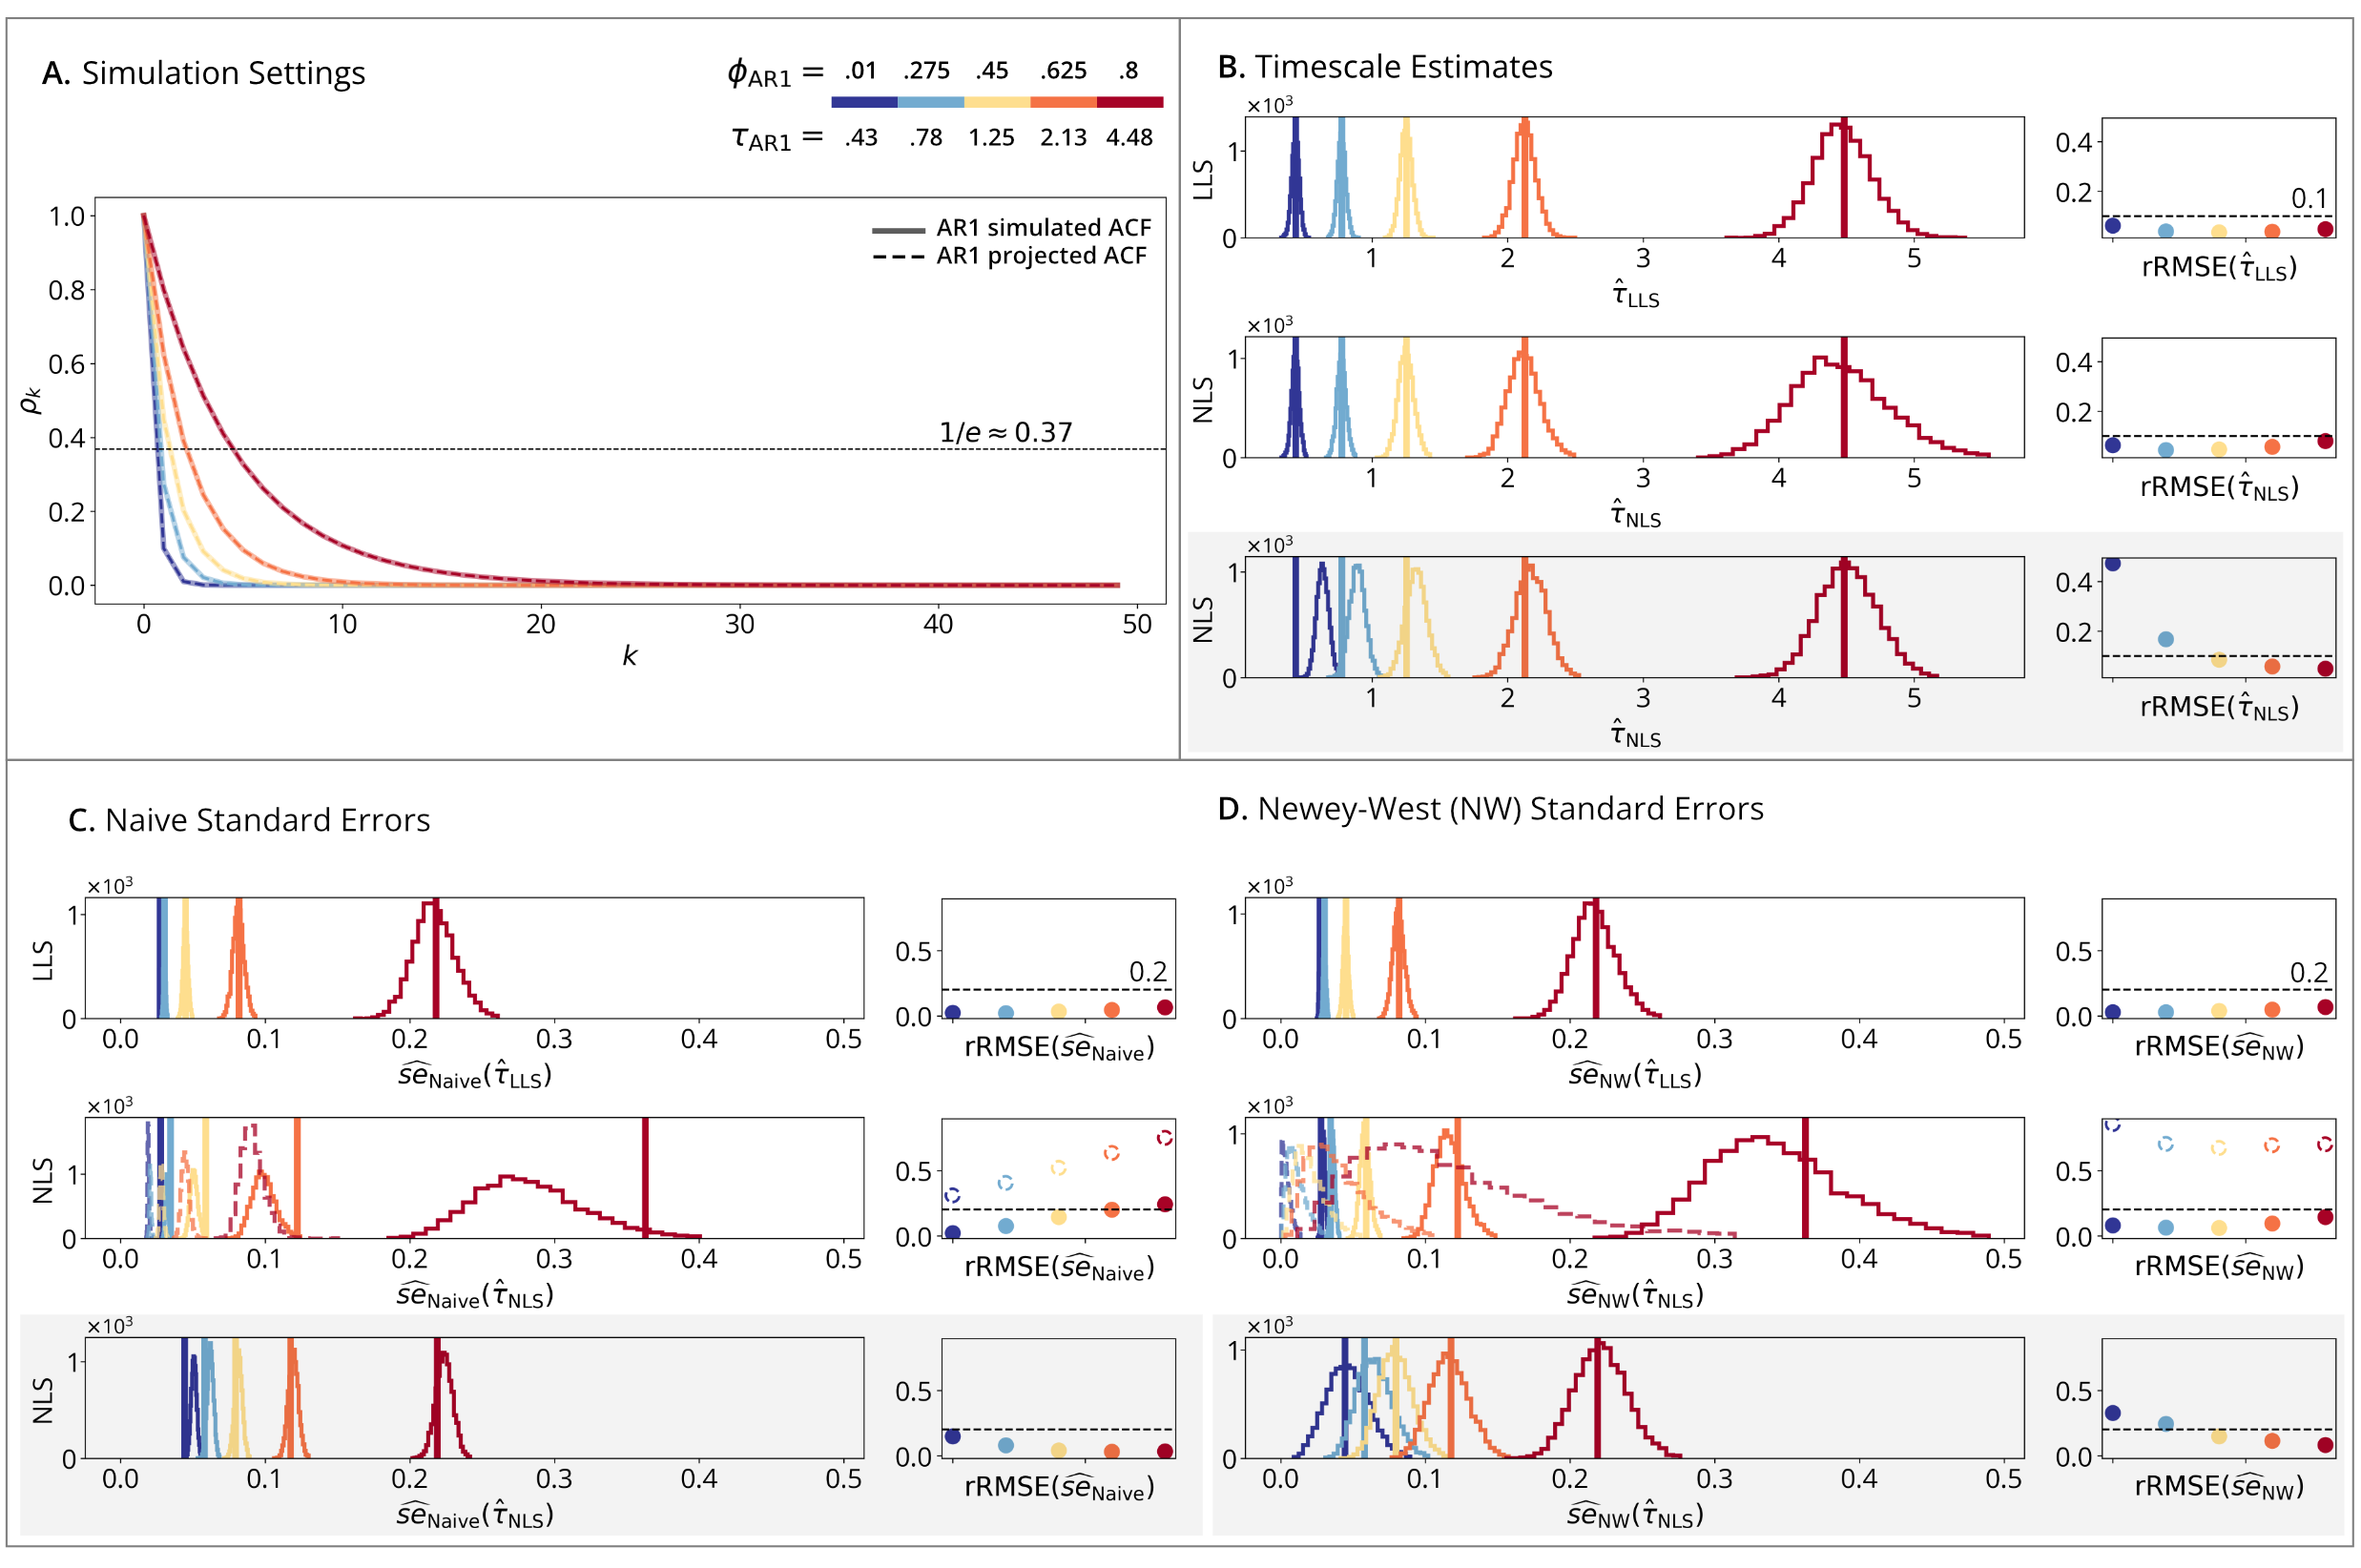
\includegraphics[width=1\textwidth]{latex/figures/fig01-ar1.png} 
    \caption{\textit{AR1 simulations.}}
    \subcaption*{
    (\textbf{A}) Simulation Setting: solid lines show the simulated ACFs; dashed lines show the AR1-projected ACFs, which are overlapping as both follow AR1. Horizontal line marks the timescale where the AR1-projected ACF reaches $1/e \approx 0.37$.
    (\textbf{B}) Timescale Estimates: vertical lines show true timescales; histograms show estimates across $N=10,000$ replications; points show rRMSE versus a 10\% error line. (\textbf{Row 1}): LLS estimator fit to time-series data. (\textbf{Row 2}): NLS estimator fit to sample ACFs from time-series data. (\textbf{Row 3}): NLS estimator fit to theoretical ACFs with added noise, which is grayed out to indicate it is not a realistic setting. (\textbf{C}) Naive and (\textbf{D}) Newey-West Standard Errors: vertical lines show standard deviations from panel B; histograms show standard error estimates; points show rRMSE versus a 20\% error line. (\textbf{Row 1}): time-domain standard errors fit to time-series data. (\textbf{Row 2} dashed lines): autocorrelation-domain standard errors fit to sample ACFs from time-series data. (\textbf{Row 2} solid lines): autocorrelation/time-domain standard errors fit to time-series data. (\textbf{Row 3}): autocorrelation-domain standard errors fit to theoretical ACFs with added noise.
    }
    \label{fig:sim-ar1}
\end{figure}

\begin{figure}[!ht]
    \centering
    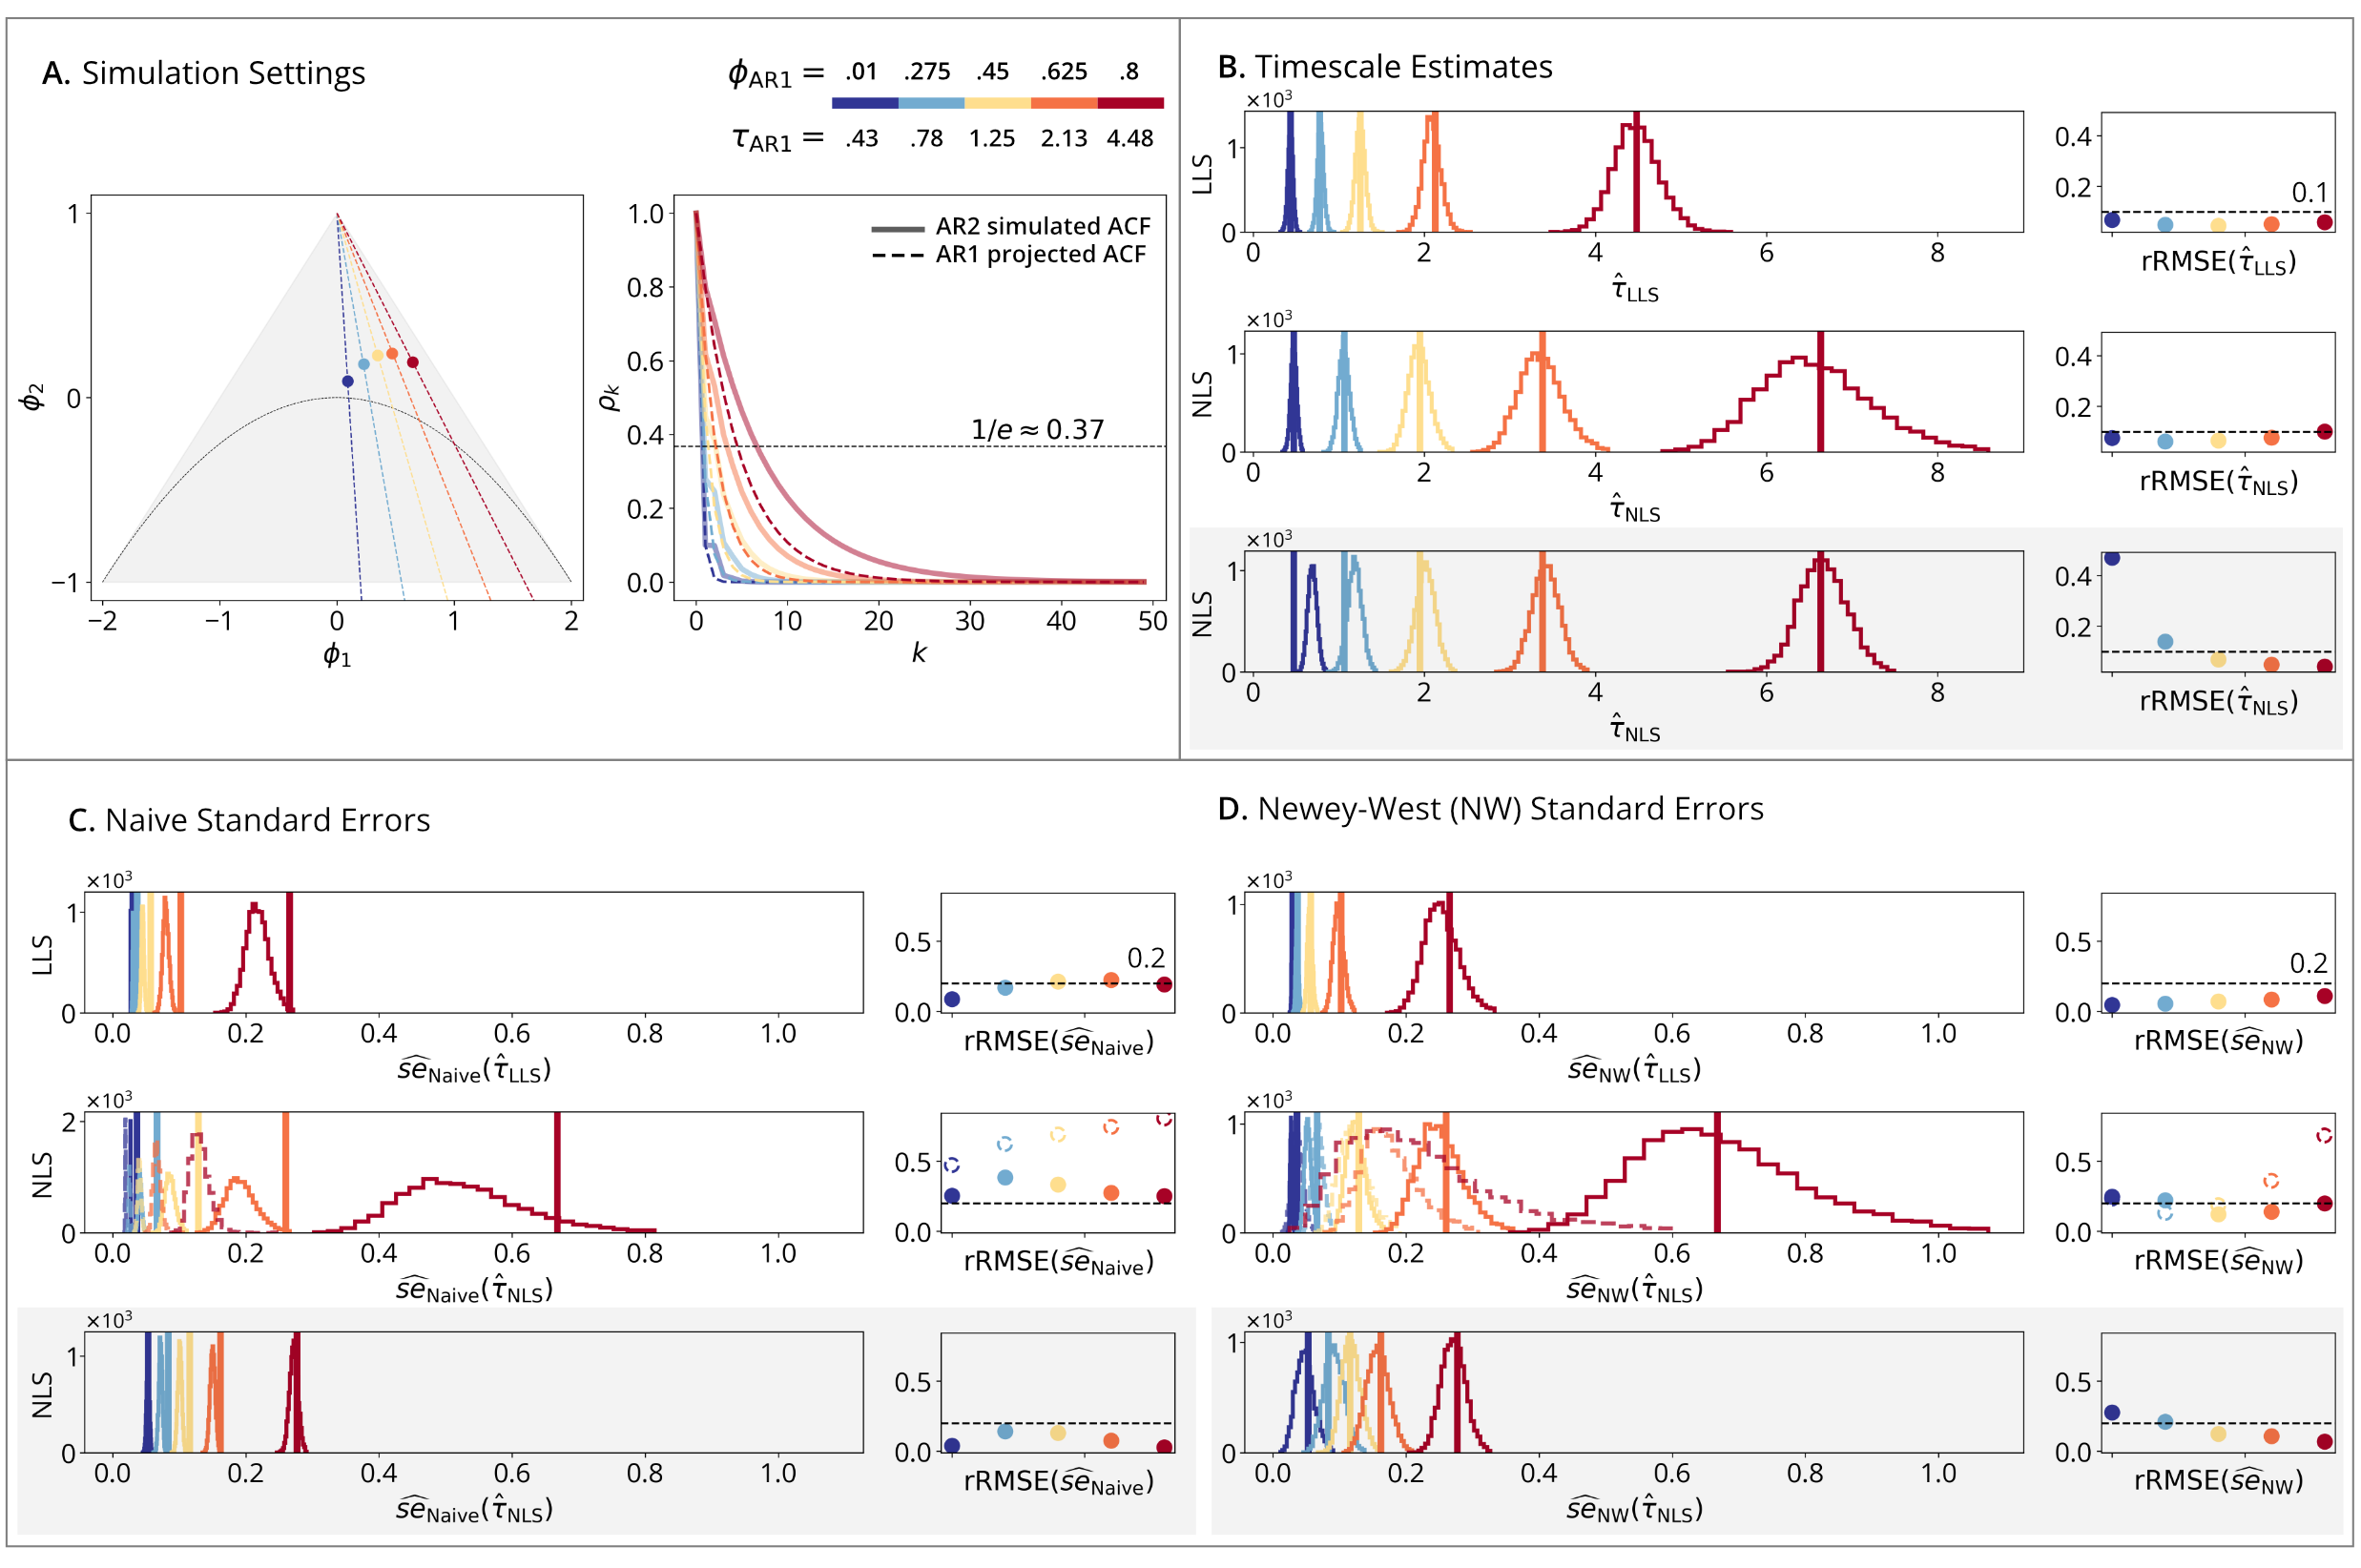
\includegraphics[width=1\textwidth]{latex/figures/fig02-ar2.png} 
    \caption{\textit{AR2 simulations.}}
    \subcaption*{
    (\textbf{A}) Simulation Setting: triangle shows AR2 stationary region in the $(\phi_1, \phi_2)$ plane with a periodic/aperiodic boundary at $\phi_2 = -\phi_1^2/4$. Points show five AR2 $(\phi_1, \phi_2)$ pairs with AR1 projections given by the colorbar. Solid lines show the simulated ACFs; dashed lines show the AR1-projected ACFs, which are not overlapping because the simulated AR2 is different from the fitted AR1.  
    (\textbf{B}) Timescale Estimates: vertical lines show true timescales; histograms show estimates across $N=10,000$ replications; points show rRMSE versus a 10\% error line. (\textbf{Row 1}): LLS estimator fit to time-series data. (\textbf{Row 2}): NLS estimator fit to sample ACFs from time-series data. (\textbf{Row 3}): NLS estimator fit to theoretical ACFs with added noise. (\textbf{C}) Naive and (\textbf{D}) Newey-West Standard Errors: vertical lines show standard deviations from panel B; histograms show standard error estimates; points show rRMSE versus a 20\% error line. (\textbf{Row 1}): time-domain standard errors fit to time-series data. (\textbf{Row 2} dashed lines): autocorrelation-domain standard errors fit to sample ACFs from time-series data. (\textbf{Row 2} solid lines): autocorrelation/time-domain standard errors fit to time-series data. (\textbf{Row 3}): autocorrelation-domain standard errors fit to theoretical ACFs with added noise.
    }
    \label{fig:sim-ar2}
\end{figure}


\begin{figure}[!ht]
    \centering
    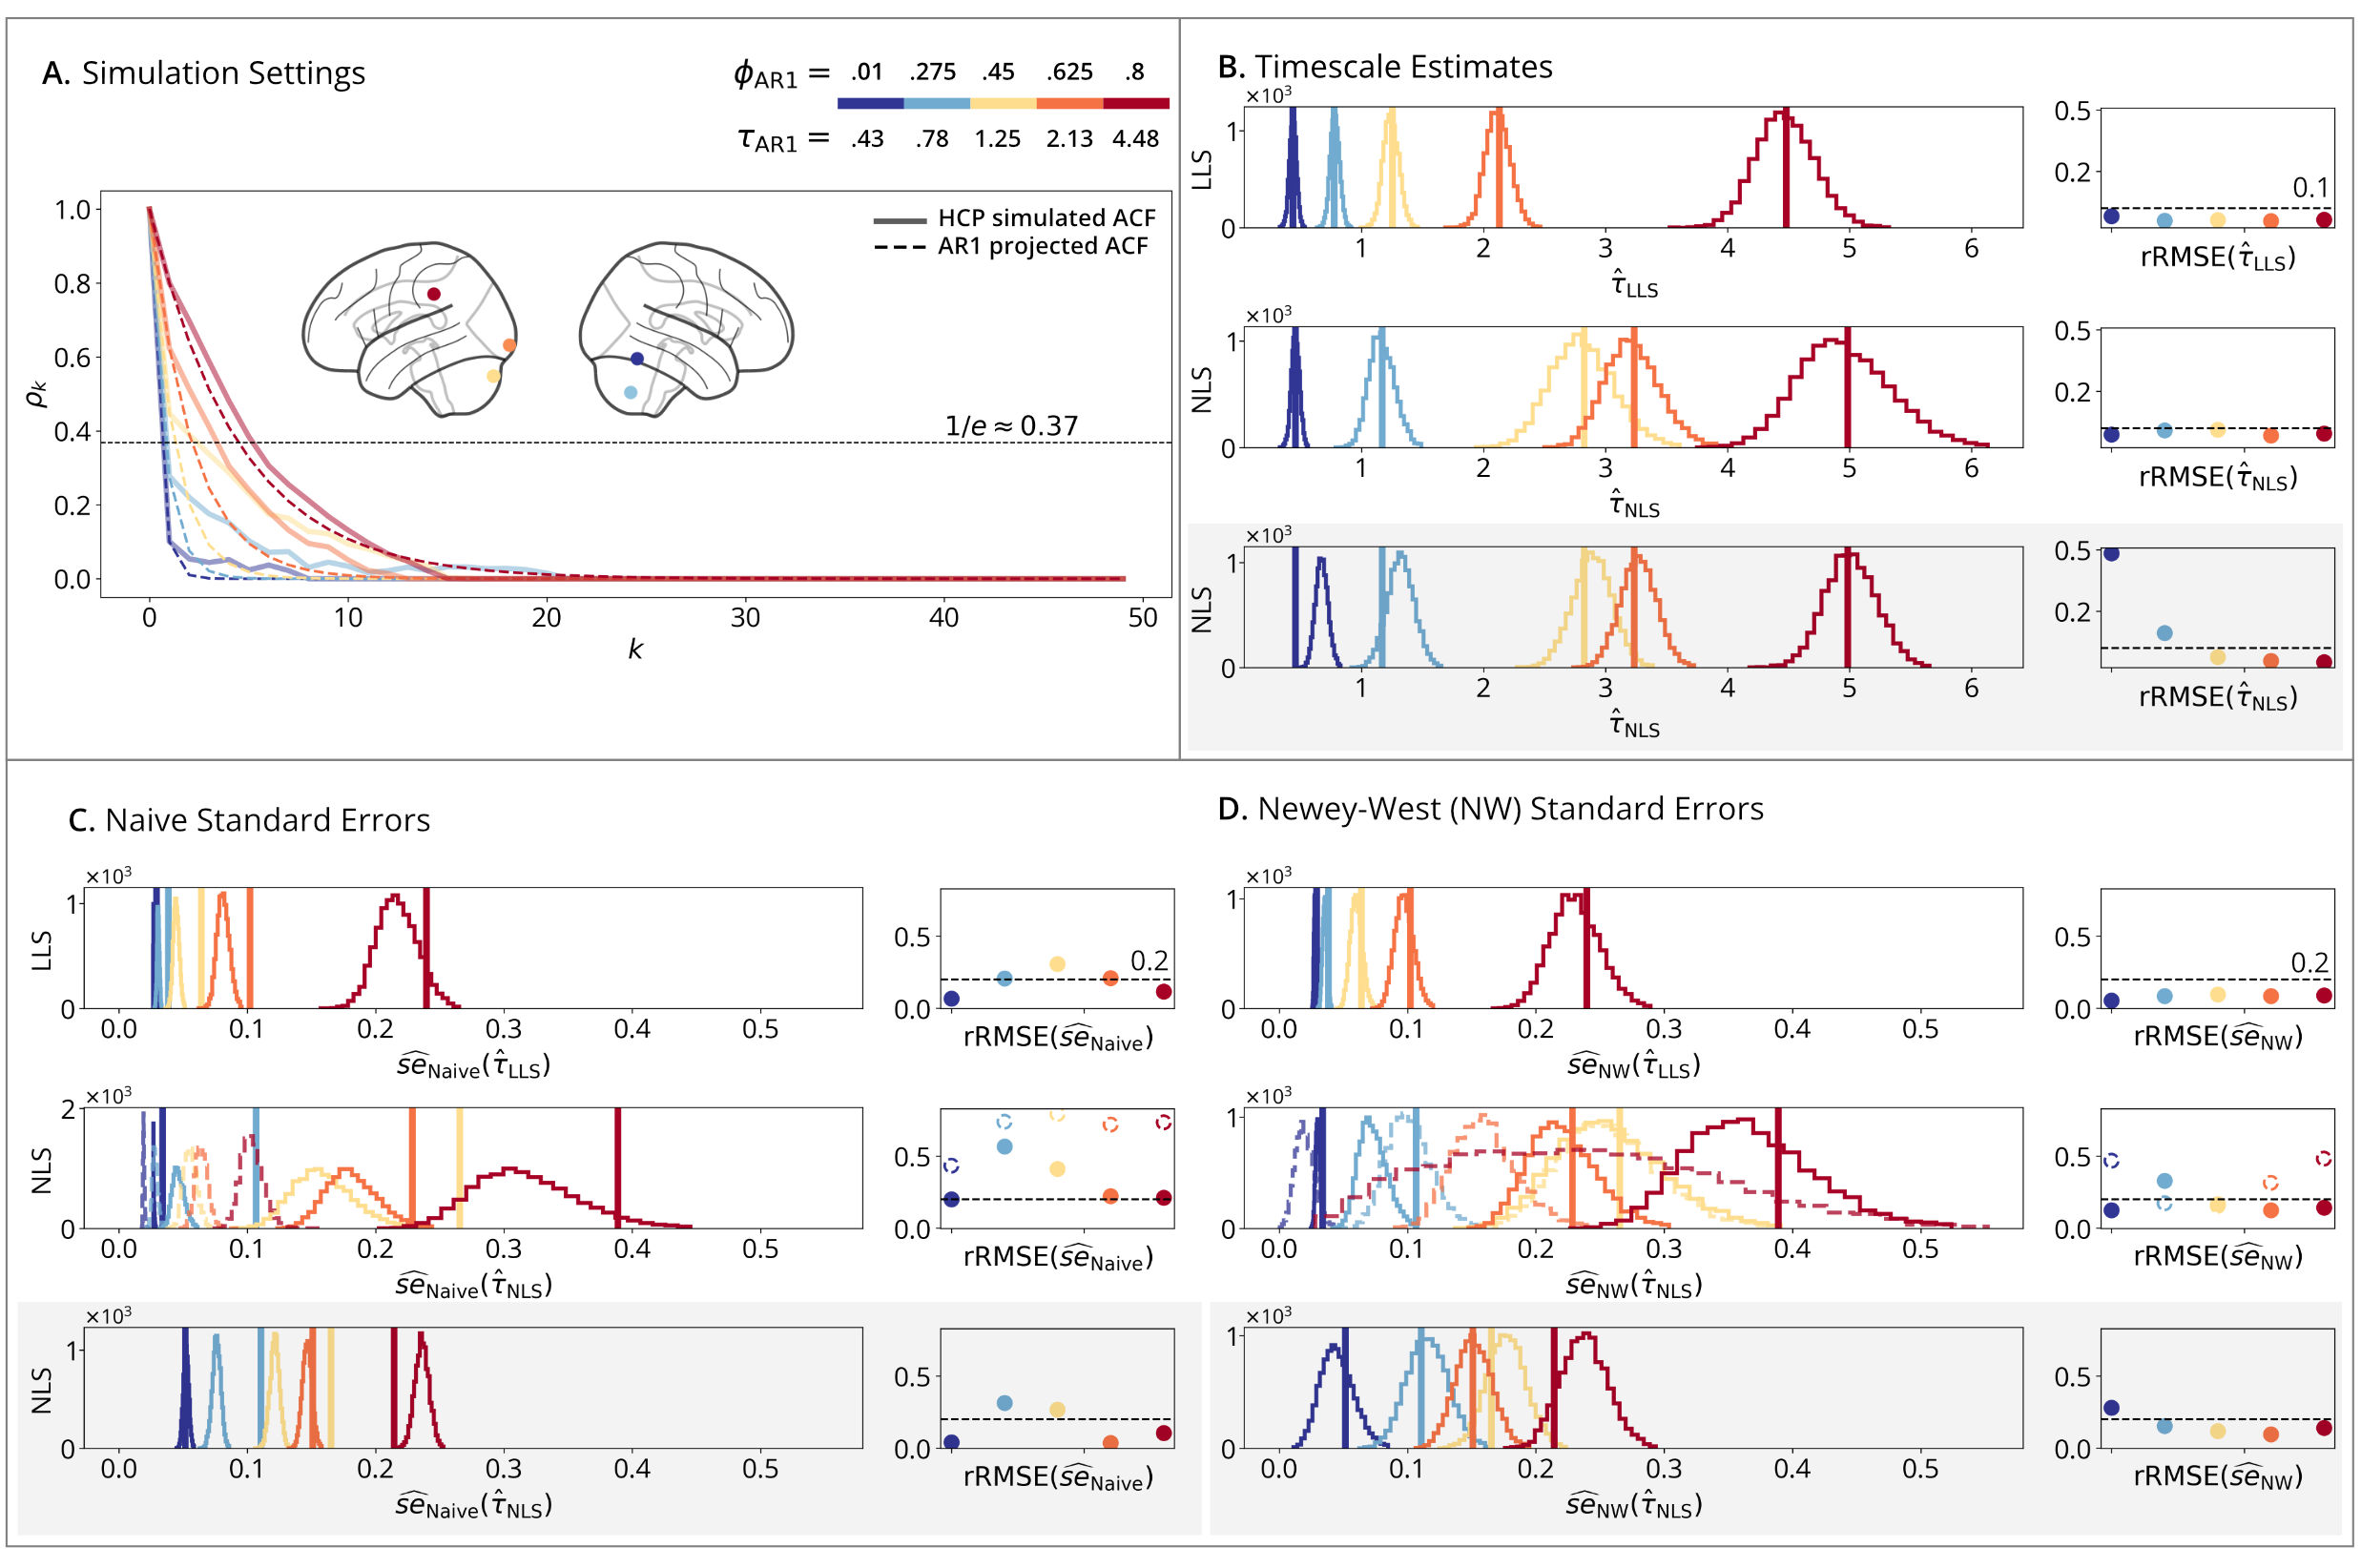
\includegraphics[width=1\textwidth]{latex/figures/fig03-hcp.png} 
    \caption{\textit{Realistic rfMRI simulations.}}
    \subcaption*{
    (\textbf{A}) Simulation Setting: solid lines show simulated ACFs from five brain regions of HCP subject $\#100610$; dashed lines show the AR1-projected ACFs, which do not overlap. 
    (\textbf{B}) Timescale Estimates: vertical lines show true timescales; histograms show estimates across $N=10,000$ replications; points show rRMSE versus a 10\% error line. (\textbf{Row 1}): LLS estimator fit to time-series data. (\textbf{Row 2}): NLS estimator fit to sample ACFs from time-series data. (\textbf{Row 3}): NLS estimator fit to theoretical ACFs with added noise. 
    (\textbf{C}) Naive and (\textbf{D}) Newey-West Standard Errors: vertical lines show standard deviations from panel B; histograms show standard error estimates; points show rRMSE versus a 20\% error line. (\textbf{Row 1}): time-domain standard errors fit to time-series data. (\textbf{Row 2} dashed lines): autocorrelation-domain standard errors fit to sample ACFs from time-series data. (\textbf{Row 2} solid lines): autocorrelation/time-domain standard errors fit to time-series data. (\textbf{Row 3}): autocorrelation-domain standard errors fit to theoretical ACFs with added noise.
    }
    \label{fig:sim-hcp}
\end{figure}

\subsubsection{Results for Autoregressive Simulations}

AR1 simulations (\textbf{Figure \ref{fig:sim-ar1}}) are correctly specified because the data-generating process aligns with the fitted models, where each time series is generated from a AR1 process and each ACF by an exponential decay (\textbf{Panel A}). \textbf{Panels B-D} show how accurately the timescale estimators recover the true parameters and their standard errors as the timescale increases. \textbf{Panel B} shows larger timescales increase estimate variability, but maintain a relative RMSE below 10\% (except that NLS shows an upward bias at small timescales in the ACF + noise setting in \textbf{panel B row 3}). \textbf{Panels C-D row 1} shows minimal difference in naive versus Newey-West standard errors under correct specification, and both give accurate estimates. \textbf{Panels C-D row 2} (dashed lines) illustrate the \nameref{sec:stderr-autocorrelation-domain_} fit to sample ACFs from time-series data, showing that both naive and Newey-West standard errors are underestimated with high rRMSE. This occurs because the method incorrectly assumes a signal + noise ACF for an AR1 process. While the timescale estimates in \textbf{panel B row 2} remain unbiased due to the correct signal specification, the standard errors are biased toward zero because the model introduces variability that is absent in the true process. \textbf{Panels C-D row 2} (solid lines) show that this variability is present in the time domain, allowing the \nameref{sec:stderr-autocorrelation/time-domain_} to uncover true standard errors, particularly for the Newey-West estimator with less than 20\% error. Finally, \textbf{panels C-D row 3} show that when the data are generated from AR1 ACFs with added noise, then the \nameref{sec:stderr-autocorrelation-domain_} accurately estimates standard errors.\\

AR2 simulation results (\textbf{Figure \ref{fig:sim-ar2}}) explore how timescale estimators perform when the data-generating process is AR2, introducing misspecification since the estimators fit AR1 projections. In this setting, the goal is to assess the impact of specification error on timescale estimation. \textbf{Panel A} illustrates the AR2 ACF and its AR1 projection, emphasizing the mismatch between the true and fitted models. \textbf{Panel B} shows that the true timescale differs between the two estimators due to their respective definitions. Despite misspecification, both timescale estimators remain mostly unbiased (except that NLS shows an upward bias at small timescales in the ACF + noise setting). \textbf{Panel C} illustrates underestimation of standard errors by the naive estimator across all time- and autocorrelation-domain methods, where the downward bias is corrected by the Newey-West standard errors of \textbf{Panel D}. As with the AR1 results, \textbf{panels C-D row 2} (dashed lines) show that the \nameref{sec:stderr-autocorrelation-domain_} fit to sample ACFs from time-series data have high rRMSE and the true standard errors are unrecoverable at large timescales even with the Newey-West approach -- another example that ACFs of AR processes cannot be represented as signal + noise models. \textbf{Panels D row 2} (solid lines) show that the \nameref{sec:stderr-autocorrelation/time-domain_} is unbiased, as with  \textbf{panel D row 3} for data generated from AR2 ACFs with added noise.


\subsubsection{Results for Realistic rfMRI Simulations}

Realistic rfMRI simulations (\textbf{Figure \ref{fig:sim-hcp}}) explore the performance of timescale estimators when simulating empirical processes derived from five distinct brain regions from a single subject. Like the AR2 results described above, this simulation method is designed to test estimator performance under model misspecification, as the data-generating process reflects realistic brain dynamics, while the fitted models project a simpler AR1 process. \textbf{Panel A} shows the mismatch between empirical ACFs and AR1 projections. \textbf{Panel B} presents the timescale estimates, where the LLS and NLS estimators yield different timescales due to their respective definitions. \textbf{Panels C-D} demonstrate that naive standard errors are underestimated; these errors are largely corrected by applying the Newey-West method. As with the AR simulations, the \nameref{sec:stderr-autocorrelation-domain_} approach is effective only when data are generated from ACFs with added noise. Otherwise, standard errors are only accurate when fit in the time domain, regardless of the domain used for timescale estimation. These results are consistent with the AR2 simulations using more realistic settings.\\

These figures highlight differences in finite sample bias and variance between the time- and autocorrelation-domain methods. (1) All timescale estimators yield largely unbiased results, while LLS performs as well or better than NLS in terms of rRMSE. (2) Standard error estimates show pronounced differences between naive and Newey-West methods for misspecified settings (AR2, realistic rfMRI). (3) Standard errors cannot be estimated in the autocorrelation domain from sample ACFs of time-series data, and require a hybrid \nameref{sec:stderr-autocorrelation/time-domain_}. (4) Time-domain methods perform as well or better than any of the autocorrelation-domain methods across all simulation results. 

\end{document}